\documentclass[11pt]{article}
\usepackage{common}
\usepackage{hyperref}
\title{Counterfactual Regret Minimization for Kuhn and Hold'em Poker}
\author{Elana Simon, Kazuma Makihara, Jack Dent}
\begin{document}
\maketitle{}


\section{Introduction}

We created a bot to play poker by implementing Counterfactual Regret Minimization (CFRM), an algorithm that has historically performed very well at poker, and that will provably converge to the game’s Nash equilibrium as the number of iterations goes to infinity. The inspiration for this bot and the proof of its correctness is given in a paper published by Todd W. Neller and Marc Lantot titled ``An Introduction to Counterfactual Regret Minimization". Our CFRM algorithm is largely adapted from the descriptions and pseudocode given in this paper.

CFRM attempts to find a strategy that minimizes the average regret over the actions for all previous iterations. The algorithm remembers which actions lead to better outcomes, and assigns positive or negative regret to these actions. It then picks an action stochastically with a probability proportional to its regret, with positive regret leading to better outcomes.

CFRM is specifically used to “solve” games. As mentioned above, CFRM uses a system of “regret matching” to track regret on certain actions, selecting each action with probability proportional to its regret. CFRM has seen particular success in poker competitions, where there is a high level of uncertainty with regard to what opponents will do, and what state the AI will begin in.

Our bot was initially implemented to play Kuhn Poker, an extremely simple version of poker involving three cards and a maximum of two rounds of betting, developed by Harold Kuhn. CFRM is a general algorithm that uses regret matching, and so can be applied to any algorithm that generates utilities, or in the terminology of CFRM, regrets. We exploited this generality by specifically coding the Kuhn poker and Hold'em implementations to return utility to a general CFRM bot. The main problem we faced technically was limiting the massive state space of Hold'em. Our bot successfully generates optimal strategies for Kuhn Poker, which has a state space of size 12. For Hold'em, we are currently using a limited deck (randomly selected 10 cards), and our bot generates reasonably successful strategies. However, there is a risk that some of the success is due to overfitting the small data set. In the future, we plan to explore featurization as another, possibly more effective, method of reducing the Hold'em state space.

\section{Background and Related Work}
The bulk of our CFRM algorithm has been adapted from Neller and Lantot's paper\cite{introtocfrm}, as mentioned in the introduction. The paper thoroughly explores and explains the background of CFRM, beginning with an explanation of utility and regret in games. It goes on to provide several simple examples, such as rock paper scissors, and the corresponding CFRM equations and results. Finally, it segues into an actual implementation of CFRM for Kuhn Poker.

We also consulted a paper published by researchers at the University of Alberta, titled ``Regret Minimization in Games with Incomplete
Information", where they present their findings on running their own CFRM bot, albeit with a much more substantial amount of computing power\cite{regretmin}. This paper was significantly more technical and served more as a complement to Neller and Lantot's paper, rather than an actual manual for CFRM implementations.

Hold'em was implemented using Jack and Kazuma's poker experience \cite{twinrivers}.

For the potential future implementations of features, the poker hand-evaluation library called ``deuces" has given us inspiration with regards to which pieces of information constitute good feature representations for Hold'em poker.

\section{Problem Specification}

Our overarching goal is to devise an algorithm that finds the optimal strategy when playing poker. In this case, we are playing zero-sum game against an opponent with imperfect information. Poker is a very complicated game where probabilistic reasoning and behavioral analysis come into play. Many would argue that the best poker players in the world are the best at reading people, but CFRM has beaten even the world's best poker players, and has provided information against this claim.

We implemented the problem as a turn based poker game. Depending on the game (Kuhn or Hold'em), each round consists of observation and action. A player's turn involves observing the information available (board, hands, previous player's action, etc.), and taking an action. The actions are picked based on a probability distribution, initially uniform. The goal of our bot is to train itself such that it returns the most effective policy, given by a probability distribution, for ensuring its own victory.

\section{Approach}

We keep a running list of our strategies for each given state, then train the bot to play the game against itself repeatedly such that each time it finishes game, it evaluates each decision it made along the way and computes the regret for each action it could have taken instead. It then updates its strategies to choose new actions based on its positive regrets of not having chosen them in the past. 

Our main data structure is a dictionary of nodes where the keys are information sets and the corresponding values are the strategy profiles. Each information set consists of all the information a player has at a given state in the game: the cards on the table, the cards in the player’s hand, and the plays that have been made so far. After a training cycle is completed, the new dictionary of information sets and strategy profiles is outputted to a text file called \texttt{strategy.txt}. The bot then uses a simple dictionary look-up at each corresponding decision point during a game to find its optimal strategy.

A strategy $\sigma_i^t$ for player $i$ after $t$ training iterations is the ``strategy profile'' or ``policy'' for player $i$ such that, for each possible state, it provides the probability of choosing each one of the possible actions. As we train, we constantly update these probabilities using the positive regrets of not taking certain actions. With each iteration through the game, we define the regret of not taking action $a$ after history $h$ as the difference between the value of the state that was reached by following the current strategy, and the value of the state that would’ve been reached by choosing action $a$. The value of a state is the sum of the utilities of all possible terminal states that can be reached given the history, weighted by the probability of reaching that terminal state.

Because our regrets are updated each time a player is in a given state, we define the cumulative counterfactual regret for an action given an information set to be the sum over all regret ever had for that action while in the state of that information set. If a given information set has any positive cumulative regrets, the strategy will be proportional to those, otherwise it will be uniform.

To formalize this, we can define state value, regret, using the equations from Neller and Lanctot paper where Z is the set of all terminal game histories, $u_i(z)$ is the utility of player i at terminal history z, $\pi^{\sigma}(I)$ is the probability of reaching information set I with strategy $\sigma$, $\pi_{-i}^{\sigma}(I)$ is the probability of counterfactually reaching information set I, so it is just the probability of reaching that information set with strategy $\sigma$ where the actions player i took to reach this state have probability 1, and $R_i^{T,+}(I,a)$ is the positive cumulative regret of player i not choosing action a at information set I. Given these definitions, the equations are:

\begin{align}
v_i(\sigma, h) &= \sum_{z \in Z, h \in z} \pi_{-i}^{\sigma}(h) \pi^{\sigma}(h,z)u_i(z)\\
r(I,a) &= \sum_{h \in I} v_i(\sigma_{I\rightarrow a}, h) - v_i(\sigma, h)\\
R_i^T(I,a) &= \sum_{t=1}^T r_i^t(I,a)\\
\sigma_i^{T+1}(I,a) &= \left\{
                \begin{array}{ll}
                  \frac{R_i^{T,+}(I,a)}{\sum_{a\in A(I)} R_i^{T,+}(I,a)},& if \sum_{a\in A(I)} R_i^{T,+}(I,a) > 0 \\
                  \frac{1}{|A(I)},& otherwise
                \end{array}
              \right.
\end{align}

\begin{algorithm}
  Initialize cumulative regret tables: $\forall I, r_I[a] \gets 0$ \\
  Initialize cumulative strategy tables: $\forall I, s_I[a] \gets 0$ \\
  Initialize initial profile: $\forall players, \sigma_{player}^1(I, A) \gets 1/|A(I)|$ \\
  \begin{algorithmic}
    \Function{CFR}{$history, cards, p0, p1$}
    \State{$player = $ current player given $history$}
    \If{$history$ is terminal}
        \State{$\textbf{return} u_{player}(history, cards)$}
    \EndIf
    \State{Let $I$ be the information set containing $history$}
    \State{$v_{\sigma} \gets 0$}
    \State{$v_{\sigma_{I \gets a}}[a] \gets 0$ for $a \in A(I)$}
    \For{$a \in A(I)$}
        \If{$player == 0$}
            \State{$v_{\sigma_{I \gets a}}[a] \gets -CFR(history + a, cards, p0 * \sigma_{player}^t(I, a), p1)$}
        \ElsIf{$player == 1$}
            \State{$v_{\sigma_{I \gets a}}[a] \gets -CFR(history + a, cards, p0, p1 * \sigma_{player}^t(I, a))$}
        \EndIf
    \State{$V_{\sigma} \gets V_{\sigma} + \sigma_{player}^t(I, a) * v_{\sigma_{I \gets a}}[a]$}
    \EndFor
    \For{$a \in A(I)$}
        \State{$regret \gets v_{\sigma_{I \gets a}}[a] - v_{\sigma}$}
        \If{$player == 0$}
            \State{$r_I{a} \gets r_I{a} + p1 * regret$}
        \ElsIf{$player == 1$}
            \State{$r_I{a} \gets r_I{a} + p0 * regret$}
        \EndIf
    \EndFor
    \State{$\textbf{return}$ $v_{\sigma}$}
    \EndFunction
    \\
    \Function{Train}{$iterations$}
        \State{$i = 0$}
        \While{$i \le iterations$}
            \State{$cards =$ random sample of cards}
            \State{$CFR(\emptyset, cards, 1, 1)$}
            \State{$i \gets i + 1$}
        \EndWhile{}
    \EndFunction
  \end{algorithmic}
  \caption{Counterfactual Regret Minimization.}
\end{algorithm}

\subsection{Limiting the State Space}

The number of possible game states in Hold'em poker is incredibly large. Indeed, for No Limit Hold'em, the state space is infinite and as such, most existing CFRM bots have only been trained on Fixed-Limit Hold'em poker. Given the limitations to our time and our computing power, we needed to reduce the size of the state space even further. Our first choice was to restrict our game to only two players. We also decided that players should be allowed to bet at most one chip per ``round" of betting. Each ``round'' starts, in our terminology, when a new card appears, or in poker a new ``round'' of betting starts on the flop, the turn, and the river. One implication of this restriction is that our game does not allow re-raises. Even ignoring betting, however, the number of possible cards draws for a two player game is approximately $10^{14}$, which is still clearly very large as a lower bound on our state space. Thus, we knew that unless our CFRM trainer ran incredibly efficiently, we would probably have to make further restrictions. 

After empirically testing our CFRM code, we found that each hand took $O(seconds)$ to train, which meant that we needed to either a) find a way to reduce the GPU time of the trainer, or b) further restrict the size of the state space. Firstly, we explored whether we could make any optimizations to reduce the time taken to train each hand. Unfortunately, it did not seem like optimization would be a sufficient strategy. We explored the possibility of leveraging Python frameworks that perform fast operations over vectorized data through C extensions such as SciPy and NumPy, but this would have required re-framing the problem in terms of matrix operations. Given that our core data structure is a game tree, we did not see how there was much scope for introducing linear algebra. For similar reasons, we did not think that GPUs would be of particular help in improving efficiency. 

\subsection{Parellelization}

Our second option was to parallelize the task bot by breaking up the CFRM trainer’s workload into lots of smaller, independent tasks. We knew that if we could find a way to shard the data according to certain requirements, we could improve the efficiency of our CFRM algorithm by training an independent bot on each shard. On a single machine, we would be able to leverage all available cores, and given access to a computing grid, we could distribute the workload across multiple machines. In other words, we wanted to make our trainer ``embarrassingly parallel''. An appropriate sharding scheme would need to adhere to a number of requirements. Firstly, we wanted to be able to specify the number of shards, so that we could reduce the total time to train the CFRM bot in proportion to the amount of computing power available. Secondly, we required that the distribution of work across shards should be uniform. As a strawman, we considered the case where one shard was given all the work, which would clearly not parallelise or improve the efficiency of our trainer. Finally, we noted that tasks should be independent, i.e. the regrets generated by a bot for a single shard should be equal to the regrets that would have been generated had there only been one shard.

We concluded that our sharding function, so as not to affect the learned regret values, should only take into account the flop cards, the number of shards, and the specific shard index. To calculate whether a given shard should learn the regret values for a given flop, we therefore used the following function:

\begin{algorithm}
  \begin{algorithmic}
    \Procedure{ShouldLearn}{$num\_shards$, $shard\_index$, $flop$}
    \State{$h = hash(flop)$}
    \State{$\textbf{return}$ $h \mod n = i$}
    \EndProcedure{}
  \end{algorithmic}
  \caption{Here is the algorithm.}
\end{algorithm}

This sharding scheme dos not affect the learned regret values, since it does not restrict the possible options for the other player’s hand, so we train against all outcomes for that flop. It also gives us a reasonable upper bound on the number of shards for a 52 card deck, $\binom{52}{3} = 22,100$.

To combine the results of training across all shards, we concatenated the output from the CFRM trainers for each shared by running \verb+cat strategy_*.txt+.

\section{Experiments}

Apart from implementing a bot that played poker according to CFRM, we also implemented a number of other basic agents to test our bot against other baseline strategies. By structuring our project to allow any two agents to compete against one another, so long as they implemented an abstract ``Agent class'', we were able to compare the performance of our CFRM bot against a number of different agents and obtain standardized performance figures across all tests.

\subsection{Kuhn Poker}

For Kuhn poker, we implemented:

\begin{enumerate}
\item ``BetAgent'', which always bets, no matter what action the opponent takes;
\item ``SimpleAgent'', which bets if it has the king, and one quarter of the time that it has the jack or the queen;
\item ``TrainedAgent'', which plays according to the results of our CFRM trainer; and
\item ``InteractiveAgent'', which delegates its choices to the command-line interface.
\end{enumerate}

To test the performance of our CFRM algorithm for Kuhn poker, after training we ran our ``TrainedAgent'' against the ``SimpleAgent'', tracking the overall number of wins and losses for each bot. Our results are described below. We varied both the number of times we trained our bot, as well as the total number of games played.

\subsection{Hold'em Poker}

For Hold'em poker, we implemented:

\begin{enumerate}
\item ``RandomAgent'', which always bets, no matter what action the opponent takes;
\item ``InteractiveAgent'', which delegates its choices to the command-line interface; and
\item ``TrainedAgent'', which plays according to the results of our CFRM trainer.
\end{enumerate}

To test the performance of our CFRM algorithm for Hold'em poker, after training we ran our ``TrainedAgent'' against the ``RandomAgent'', also tracking the overall number of wins and losses for each bot. Our results are described below.

\subsection{Results}
Below, we have a table and graph of our trained bot's performance against the simple bot described above, playing games of Kuhn poker. The $x$ axis represents the number of iterations our bot was trained for (the number of times we ran our CFRM algorithm), and the $y$ axis is the percentage of times our trained bot won against the simple bot.

As shown, when the number of iterations is low, the data is very volatile. This is to be expected, since the fewer the iterations, the less accurate the data is. For example, if the bot happens to lose on a hand where the probability of winning should be high, an early strategy will bias towards the loss rather than internalizing it as the number of iterations increases. As the number of iterations increases exponentially, the bot approaches a success rate of 94\%.

\begin{table}
\centering
    \begin{tabular}{|l|l|}
    \hline
    \textbf{Number of training iterations} & \textbf{Percentage of games won} \\ \hline
    1 & 66 \\ \hline
    10 & 99 \\ \hline
    50 & 96 \\ \hline
    100 & 57 \\ \hline
    200 & 86 \\ \hline
    500 & 84 \\ \hline
    1000 & 71 \\ \hline
    2000 & 86 \\ \hline
    5000 & 90 \\ \hline
    10000 & 91 \\ \hline
    50000 & 92 \\ \hline
    100000 & 92 \\ \hline
    1000000 & 94 \\ \hline
    5000000 & 94 \\ \hline
    \end{tabular}
\end{table}

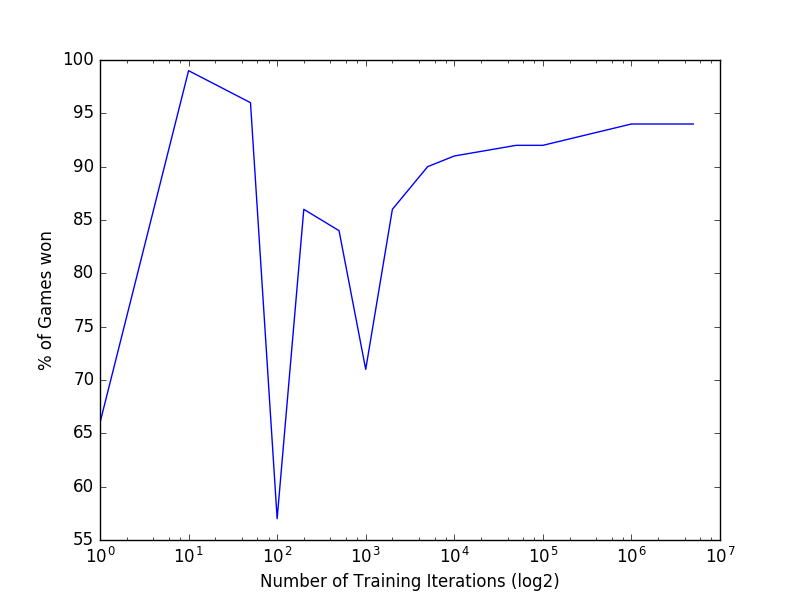
\includegraphics[scale=0.75]{KuhnResults} \\

As mentioned before, Hold'em's massive state space and our limited computing power prevent us from running similar tests. When training our bot with 10 cards, the Odyssey cluster allowed us to train each state at most 4 times. Due to the randomness of how the hands and the deck are chosen (we make it random to reduce as much overfitting as possible), not every state will actually be trained. So far, we have observed that a majority of states are trained, but this is not guaranteed for the previously stated reason. Currently, our Hold'em bot beats the random bot 93\% of the time, give or take 6 percentage points. While our bot is very successful, we cannot ignore the possible effects of overfitting such a small subset of test data. However, the high numbers still are promising, and the effectiveness of the algorithm is shown through the bot's performance in Kuhn poker. We lay out what we plan to do in the future to limit the Hold'em state space and increase the algorithm's speed in the discussion section below.

\section{Discussion}

Over the course of this project, our team learned a lot more about the limitations of computing power, a very real issue that many artificial intelligence and machine learning algorithms wrestle with. With more computing power over a larger computing cluster, we would be able to increase the parrellization of the training process and ``solve'' limit Texas Hold'em (no-limit Hold'em has an infinite state space) by running our current CFRM algorithm. If we ignore betting, the state space of our limit Hold'em game is roughly $10^14$. Researchers at the University of Alberta calculated a strategy to within 1\% of an unexploitable Nash Equilibrium over several months of parallel computing on 200 machines\cite{pokernews}. Our resources were limited to our 3 computers (8 cores total) and the Harvard Odyssey cluster, which let us run a maximum of 7,500 processes concurrently. When limited to a deck of 10 randomly selected cards, we were able to train each strategy at most 4 times over the span of 5 hours. We are also not the only group using the Odyssey cluster, so were limited by the number of jobs we could send/queue.

In the future, we are looking to find other methods to limit Hold'em's massive state space. One option is featurization. This would involve classifying states and their corresponding strategies by certain features, rather than the entire information set itself (hand, board, previous actions). It is important to make the features general enough that they reduce the size of the state space, but specific enough that we don't overgeneralize and lose the algorithm's effectiveness. Among others, example features include hand types (flush, straight, pair), hand rankings within types (high pair, low pair, pairs > 10), and probability of victory. We could construct an entirely separate project simply around which features are best at generalizing a Hold'em game. We hope to continue working on this project independently as Jack and Kazuma are avid poker players, and Elana is learning.

\newpage
\appendix

\section{Appendix: System Description}

\begin{enumerate}
\item Installations 
	\begin{itemize}
    	\item Clone our repo from \boxed{\href{https://github.com/jackdent/cs182-poker}{Github Repo}}
    	\item To install deuces open a terminal and type \texttt{pip install Deuces}
    	\item To access odyssey follow the instructions at: \boxed{\href{https://rc.fas.harvard.edu/resources/access-and-login}{RC Access and Login}} (Only necessary if training Hold'em)
    \end{itemize}
\item Training
	\begin{itemize}
         \item Kuhn
         	\begin{itemize}
         		\item From the cs182-poker folder run \texttt{python -m poker.kuhn.cfrm}
                \item When prompted, type the number of iterations you wish to train, we recommend more than 1,000,000.
         	\end{itemize}
            \item Hold'em
    	\begin{itemize}
            \item We would recommend not trying to train Hold'em as it will take many hours but if you wish, you can do this by logging into odyssey and copying the cs182-poker into your environment on Odyssey. You also need to install deuces in this environment.
            \item Log in to Odyssey then run \texttt{sbatch --array=0-197 ./train\_10\_holdem.sh}
            \item If you just want to see that the trainer works, you can run \texttt{python -m poker.holdem.cfrm} and it will just run 1 training iteration. If you wish to train more you can adjust using the command line flags
         \end{itemize}
    \end{itemize}
\item Testing
	\begin{itemize}
    	\item Kuhn
    	\begin{itemize}
            \item From the cs182-poker folder run \texttt{python -m poker.kuhn.main}
            \item When prompted, type ``s'' to test the trained agent against a simple agent and ``t'' to test the agent against another trained agent
            \item The trained agent should outperform the simple agent but should approximately tie with the other trained agent.
      	\end{itemize}
        \item Hold'em
        \begin{itemize}
        	\item From the cs182-poker directory run \texttt{python -m poker.holdem.main -- test}
            \item This will take a moment to load our massive training file, then will test our trained bot against a random one 100 times and print out the total percent of games that our bot won against the random. Whereas Kuhn uses a command line prompt to specify test or play, due to the long time required to upload the training data, Hold'em uses a flag so that the testing occurs without waiting for a prompt
        \end{itemize}
    \end{itemize}
\item Playing
	\begin{itemize}
    	\item Kuhn
        \begin{itemize}
        	\item Run \texttt{python -m poker.kuhn.main} and when prompted, type ``i'' to interactively play with the agent!
        \end{itemize}
    	\item Hold'em
        	\begin{itemize}
            	\item If you run \texttt{python -m poker.holdem.main} (without the \texttt{--test}) flag it will again take a few moments 
                \item To load the test file, but then let you play against the bot yourself!
            \end{itemize}  
    \end{itemize}
\end{enumerate}

\section{Appendix: Group Makeup}
\begin{enumerate}
\item Kazuma Makihara was responsible for coding much of the CFRM algorithm itself and much of the early testing with Kuhn Poker. He also contributed to the early stage research, looking into and testing different poker implementations (Kuhn Poker vs. Leduc Hold'em), as well as research into featurization.

\item  Jack Dent was responsible for much of the initial research, proposing CFRM and finding the Neller and Lantot paper. He was also responsible for coding the Kuhn and Hold'em implementations, as well as suggesting and designing our parallel computing structure as a solution to our computing issues.

\item Elana Simon spent much of her time adapting the Hold'em code to fit the CFRM algorithm, as well as implementing the sharding scheme. She was also responsible for training the bot on the Odyssey cluster, sending jobs at all hours of the night to ensure the results were robust.

\end{enumerate}

\newpage

\nocite{*}
\bibliographystyle{plain} 
\bibliography{project}

\end{document}

